\documentclass[12pt,a4paper]{article}
\usepackage[utf8]{inputenc}
\usepackage[T1]{fontenc}
\usepackage{comment}
\date{} 
\usepackage[spanish]{babel}
\usepackage{amsmath}
\usepackage{amsfonts}
\usepackage{amssymb}
\usepackage{graphicx}
\usepackage{float} 
\usepackage{mathpazo} % Palatino font
\usepackage[left=2.50cm, right=2.50cm, top=1.50cm, bottom=1.50cm]{geometry}
\author{Caamiña, Daniela \and Yapura, Cristian}
\title{Trabajo final \\Automatización industrial}
\graphicspath{ {images/} }

	
\begin{document}
	\begin{titlepage} %Carátula 			
		\newcommand{\HRule}{\rule{\linewidth}{0.5mm}} 
		\center % Centre everything on the page		
		\textsc{\LARGE Universidad Nacional de la Patagonia San Juan Bosco}\\[1.5cm]
		\textsc{\Large Automatización Industrial}\\[0.5cm]
		\textsc{\large Trabajo Final}\\[0.5cm] 
		\HRule\\[0.4cm]
		\huge\bfseries{Banco de pruebas para motor trifásico}\\[0.2cm] 
		\HRule\\[1.5cm]
			\begin{minipage}{0.4\textwidth}
				\begin{flushleft}
					\large
					\textit{Alumnos}\\
					\textsc{Caamiña,} Daniela \\
					\textsc{Yapura,} Cristian  
				\end{flushleft}
			\end{minipage}
			\begin{minipage}{0.4\textwidth}
				\begin{flushright}
					\large
					\textit{Docentes}\\
					Ing. \textsc{Lorenc,} Marcelo \\
					Dr. \textsc{Peña,} Ramiro  
				\end{flushright}
			\end{minipage}
		\vfill\vfill\vfill 
		\large{Junio 2020} 
		\vfill\vfill
		
\includegraphics[width=0.2\textwidth]{unpsjb.png}\\[1cm] 
		\vfill 
	\end{titlepage}
	
\tableofcontents
\newpage

\listoffigures
\newpage	
		
\section{Introducción}
Actualmente en el Laboratorio de Automatización y Control de la Universidad, se cursan distintas materias en las cuales se necesitan herramientas para realizar diversas prácticas, con el fin de afianzar los conocimientos que se adquieren a lo largo del año.
\\

Para llevar a cabo estas actividades con varias etapas, se requiere demasiado tiempo en realizar pruebas sobre un esquema complejo, es decir con varios elementos, ya que se necesita armar un prototipo de banco de prueba cada vez que sea necesario. Por ejemplo, realizar la conexión de un PLC, variador de frecuencia y un motor puede ser una tarea repetitiva que se busca suprimir. 

\newpage

\section{Objetivo}
Generar un lazo de control que tenga como entrada la velocidad de referencia, y que contemple las perturbaciones externas del sistema en el cálculo de la velocidad de salida que se utilizará como lazo de realimentación. 
Adaptar la acción de control que ingresa al variador de velocidad (adquirido por el Laboratorio de Fluidos) para alimentar al motor y dejar en desuso el banco de resistencias que se utiliza.
Además, realizar una interfaz gráfica para un mejor manejo y control del sistema.

\begin{figure}[htb]
	\centering
	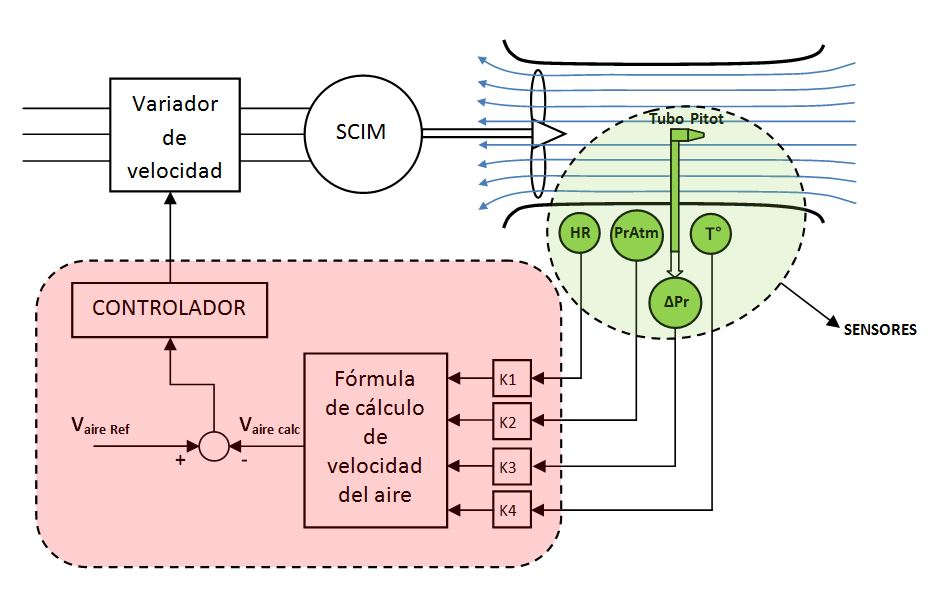
\includegraphics[scale=0.35]{diagr.jpg}
	\caption{Diagrama}
	\label{fig:diagr}
	\end{figure}
	
\section{Motor}
\subsection{Especificaciones}

	El motor (Figura \ref{fig:motor}) asincrónico que se utiliza es de la marca \textbf{Altium} perteneciente a la firma \textbf{Schneider Electric}. Las especificaciones se muestran a continuación \\
	\paragraph*{Altium Eff2}
	\begin{itemize}
		\item 	Tipo: TE2A90SP2
		\item   Tensión nominal: 220/380 V
		\item 	Corriente nominal: 5.97 A 
		\item	Frecuencia nominal:  50 Hz.
		\item 	Potencia: 1.5kW / 2 HP
		\item 	Fases: 3
		\item   Factor de Potencia: 0.84
	\end{itemize}
	\newpage
	\begin{figure}[h!]
		\centering
		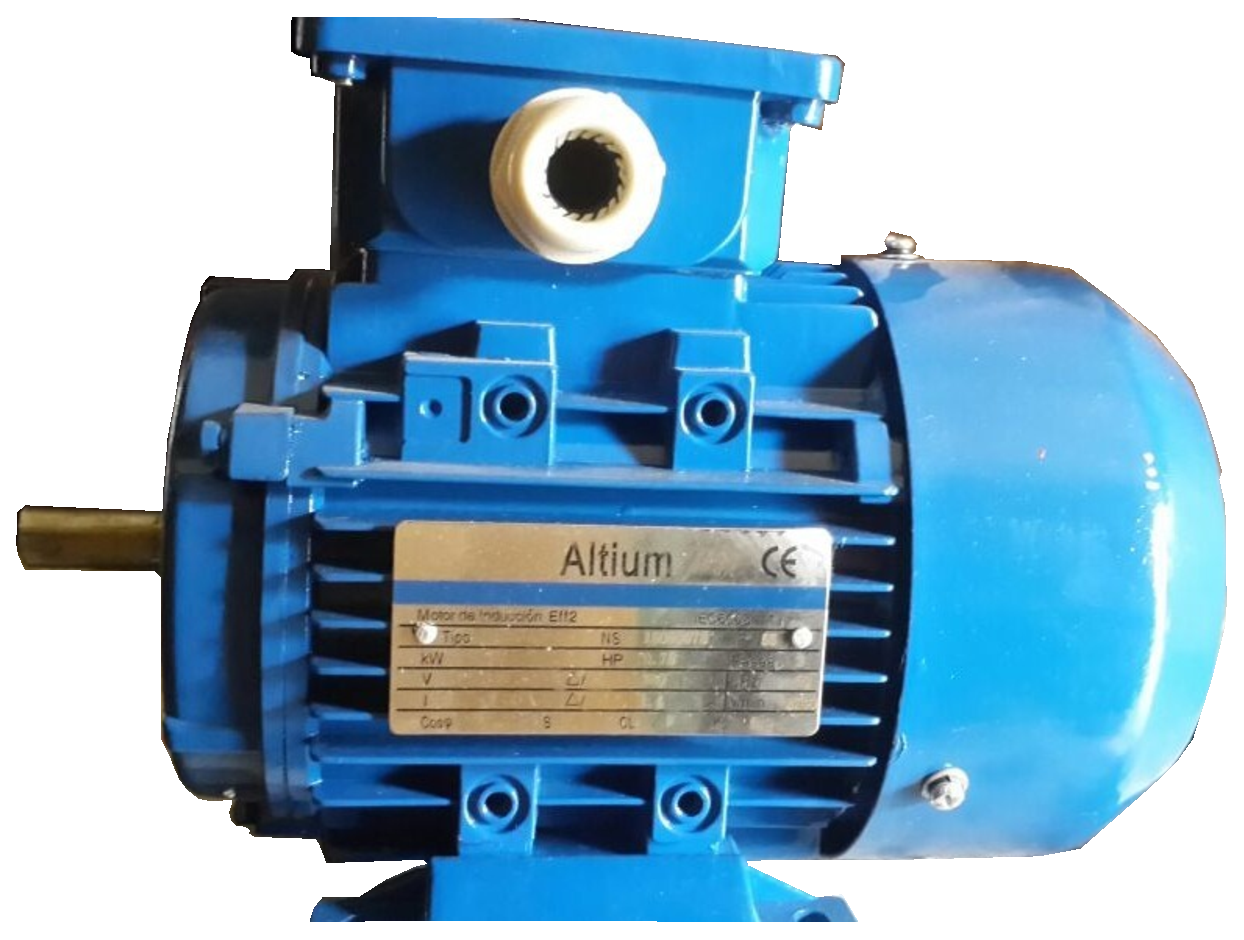
\includegraphics[scale=0.4]{motor.eps}
		\caption{Motor Altium}
		\label{fig:motor}
	\end{figure}
	\newpage

\section{Variador de velocidad}
\subsection{Especificaciones}
El variador de velocidad que se utilizó pertenece a la marca \textbf{Schneider Electric} (Figura \ref{fig:variador}) que posee las siguientes características. \\
	\paragraph*{Altivar 312}
	\begin{itemize}
		\item 	Modelo: ATV312HU15N4
		\item   Tensión: 380-500 V
		\item 	Frecuencia: 50/60 Hz
		\item 	Potencia: 1.5kW / 2 HP
		\item 	Fases: 3
	\end{itemize}

	\begin{figure}[h!]
		\centering
		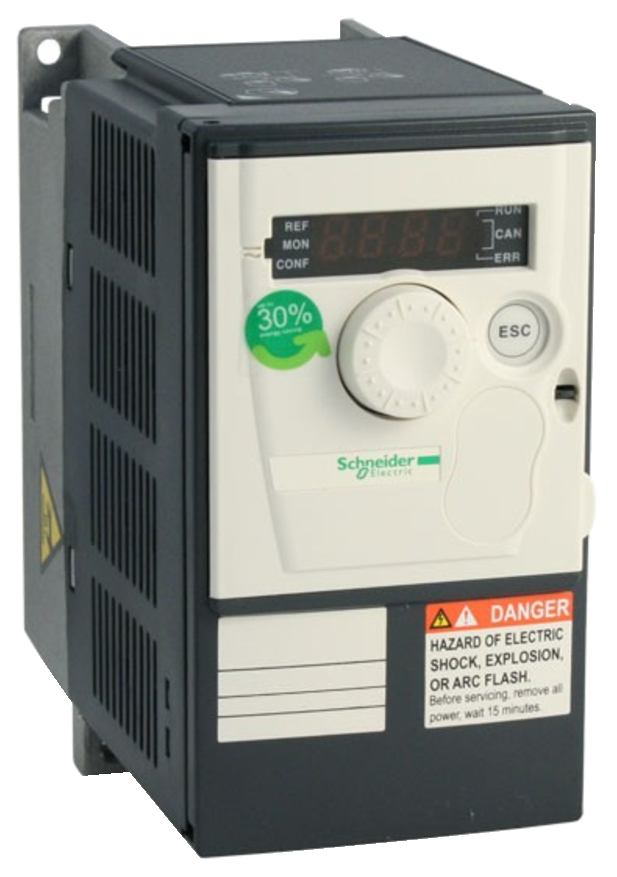
\includegraphics[scale=0.4]{variador.eps}
		\caption{Variador de velocidad Altivar 312}
		\label{fig:variador}
	\end{figure}


	\subsection{Configuración de parámetros primarios}
	Para realizar la configuración del motor se utilizó el software SoMove. Se descargó la ultima versión desde la página oficial de Schneider\footnote{\url{https://www.se.com/ar/es/product-range-presentation/2714-somove/}} y luego, la librería DTM correspondiente al variador a utilizar\footnote{\url{https://www.se.com/ar/es/download/document/Altivar_DTM_Library/}}. 
	\\
	Una vez realizado esto se procedió a generar un nuevo proyecto eligiendo las opciones correctas del variador.
	
	
	\newpage


	
\section{PLC}
\subsection{Módulos PLC M340}

EL ERROR QUE TENIA CRISTIAN con ifix SE ARREGLO CON ESTO
\url{http://www.cimexcorp.com/hasp_fix.htm}
\subsection{Especificaciones}
\subsection{Comunicación}
El   variador   también   se   puede   controlar   en   modo   remoto.   Es   adecuado   paraaplicaciones en   los   que   los   cambios   de   variables   del   variadorse   realizan frecuentemente  durante  el proceso.  Dichos  cambios  pueden  realizarse  por  parte  del propio  operario  (mediante  potenciómetros,  interruptores,  selectores  rotativos  o  BCD, etc.).  Sin  embargo,  la  situación  más  común  es  que  los  parámetros  del  variador  los establezca  el  equipo  de  control  y  supervisión  del  proceso,  al  que  está  conectado  el variadorde  frecuencia: reguladores  de  tensión  y/o  corriente,  finales  de  carrera, pantallas de operador, etc., o incluso un ordenador personal y/o PLC. Para  el  casode  estos  controles  remotos,  la  comunicación  se  puede  realizarde  dos modos:\\Mediante un  número  determinado  de  conductores,  que  depende  de  los elementos que se tengan conectados al variador de frecuencia, por el que se transmiten señales digitales (finalesde carrera, interruptores, salidas digitales de un PLC), o analógicas (potenciómetro, salida analógica de un PLC):\\Mediante un bus de comunicaciones industriales (de 2 o 4 hilos), sobre el que se transmiten   mensajes   de   ajuste   de   parámetros   siguiendo   un   protocolo preestablecido (Modbus, CanBus, ProfiBus, EtherCat, etc.).Con 2  conductores la  comunicación  se  hace  más  lenta(modo  semidúplex),  pero  lógicamente representa un menor coste.
	
\subsubsection{Diagrama}
	\begin{figure}[htb]
		\centering
		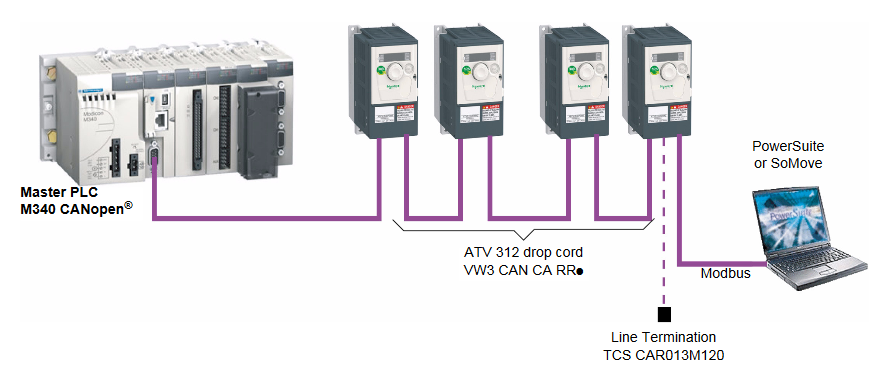
\includegraphics[scale=0.7]{comu.png}
		%\caption{Placa BME280}
		%\label{fig:BME280}
	\end{figure}	
	

\subsubsection{CANopen}
\subsubsection{Modbus}


	\newpage



	\newpage
	
\section{Banco de pruebas}
\subsection{Banco de pruebas}
\subsubsection{Elementos}
Se decidió que el banco de pruebas cuente con los siguientes elementos:
\begin{itemize}
	\item interruptor
	\item botón de marcha/ parada
	\item botón parada de emergencia
	\item señalización lumínica
	\item freno para generar perturbaciones 
	\item riel para colocar un nuevo motor que actuará como carga
	\item Panel de control
		\subitem Botón de emergencia
		\subitem Encendido/ apagado
		\subitem Potenciómetro para variar velocidad
		\subitem Display para observar velocidad
		\subitem Alarmas visuales
\end{itemize}
\subsubsection{Presupuesto--Valor--Costo a tal día}
\subsection{HMI}

Se realizó una interfaz humana maquina con los siguientes elementos:
	\begin{itemize}
		\item boton de start(acá o en el tablero???)
		\item varias velocidades configuradas previamente
		\item inversión y señalización del mismo
		\item torque???
		\item HMI
        	\subitem Alarmas
       		\subitem Información en tiempo real
        	\subitem Histórico de datos
        	\subitem Control general del banco
	\end{itemize}
	\begin{figure}[htb]
		\centering
		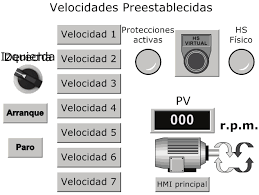
\includegraphics{HMIej.png}
		%\caption{Placa BME280}
		%\label{fig:BME280}
	\end{figure}

\newpage

\section{Comunicación}
El   variador   también   se   puede   controlar   en   modo   remoto.   Es   adecuado   paraaplicaciones en   los   que   los   cambios   de   variables   del   variadorse   realizan frecuentemente  durante  el proceso.  Dichos  cambios  pueden  realizarse  por  parte  del propio  operario  (mediante  potenciómetros,  interruptores,  selectores  rotativos  o  BCD, etc.).  Sin  embargo,  la  situación  más  común  es  que  los  parámetros  del  variador  los establezca  el  equipo  de  control  y  supervisión  del  proceso,  al  que  está  conectado  el variadorde  frecuencia: reguladores  de  tensión  y/o  corriente,  finales  de  carrera, pantallas de operador, etc., o incluso un ordenador personal y/o PLC. Para  el  casode  estos  controles  remotos,  la  comunicación  se  puede  realizarde  dos modos:\\Mediante un  número  determinado  de  conductores,  que  depende  de  los elementos que se tengan conectados al variador de frecuencia, por el que se transmiten señales digitales (finalesde carrera, interruptores, salidas digitales de un PLC), o analógicas (potenciómetro, salida analógica de un PLC):\\Mediante un bus de comunicaciones industriales (de 2 o 4 hilos), sobre el que se transmiten   mensajes   de   ajuste   de   parámetros   siguiendo   un   protocolo preestablecido (Modbus, CanBus, ProfiBus, EtherCat, etc.).Con 2  conductores la  comunicación  se  hace  más  lenta(modo  semidúplex),  pero  lógicamente representa un menor coste.
	
\subsubsection{Diagrama}
	\begin{figure}[htb]
		\centering
		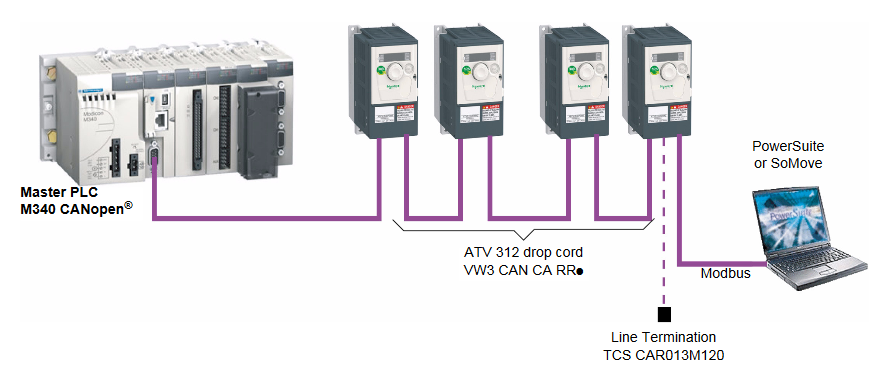
\includegraphics[scale=0.7]{comu.png}
		%\caption{Placa BME280}
		%\label{fig:BME280}
	\end{figure}	
	

\subsubsection{CANopen}
\subsubsection{Modbus}


	\newpage

\section{Conclusiones}

\newpage

\section{Anexos}
\newpage


\end{document}